%\documentclass[12pt,notitlepage]{article}
\documentclass[a4paper,12pt]{article}
\usepackage[utf8]{inputenc}
\usepackage{graphicx}
\usepackage{verbatim}
\usepackage{amsthm}
\usepackage{amssymb}
\usepackage{pdfpages}
\usepackage{amsmath}
\usepackage{tikzsymbols}
\usepackage{mathtools}
\usepackage{enumitem}
\DeclarePairedDelimiter\ceil{\lceil}{\rceil}
\DeclarePairedDelimiter\floor{\lfloor}{\rfloor}

\usepackage{hyperref}
%\usepackage[T1]{fontenc}
\usepackage{url}
\usepackage{lipsum}
\usepackage{array}
\usepackage{multirow}
\usepackage{float}
\usepackage{lscape}
\usepackage{colortbl}
\newcolumntype{P}[1]{>{\centering\arraybackslash}p{#1}}
\usepackage[nottoc,numbib]{tocbibind}
\usepackage{fancyhdr}
\usepackage{hhline}
\usepackage[printonlyused]{acronym}

%\usepackage{txfonts}
\usepackage{lipsum,etoolbox}% http://ctan.org/pkg/{lipsum,etoolbox}
\usepackage{caption}
\usepackage{subcaption}

\usepackage{algorithm}
\usepackage[noend]{algpseudocode}

\makeatletter
\def\BState{\State\hskip-\ALG@thistlm}
\makeatother

\usepackage{minted}

\definecolor{black}{RGB}{0,0,0}

\usepackage{fancyvrb}

\usepackage{geometry}
\geometry{
	a4paper,
	total={170mm,257mm},
	right=3cm,
	left=3.5cm,
	top=3cm,
	bottom=3cm
}

\makeatletter
\DeclareRobustCommand{\rvdots}{%
	\vbox{
		\baselineskip4\p@\lineskiplimit\z@
		\kern-\p@
		\hbox{.}\hbox{.}\hbox{.}
}}
\makeatother

\usepackage{titlesec}
\usepackage{hyperref}
\titleclass{\subsubsubsection}{straight}[\subsection]

\newcounter{subsubsubsection}[subsubsection]
\renewcommand\thesubsubsubsection{\thesubsubsection.\arabic{subsubsubsection}}
\renewcommand\theparagraph{\thesubsubsubsection.\arabic{paragraph}} % optional; useful if paragraphs are to be numbered

\titleformat{\subsubsubsection}
{\normalfont\normalsize\bfseries}{\thesubsubsubsection}{1em}{}
\titlespacing*{\subsubsubsection}
{0pt}{3.25ex plus 1ex minus .2ex}{1.5ex plus .2ex}

\makeatletter
\renewcommand\paragraph{\@startsection{paragraph}{5}{\z@}%
	{3.25ex \@plus1ex \@minus.2ex}%
	{-1em}%
	{\normalfont\normalsize\bfseries}}
\renewcommand\subparagraph{\@startsection{subparagraph}{6}{\parindent}%
	{3.25ex \@plus1ex \@minus .2ex}%
	{-1em}%
	{\normalfont\normalsize\bfseries}}
\def\toclevel@subsubsubsection{4}
\def\toclevel@paragraph{5}
\def\toclevel@paragraph{6}
\def\l@subsubsubsection{\@dottedtocline{4}{7em}{4em}}
\def\l@paragraph{\@dottedtocline{5}{10em}{5em}}
\def\l@subparagraph{\@dottedtocline{6}{14em}{6em}}
\makeatother
\newcommand*\circled[1]{\tikz[baseline=(char.base)]{
		\node[shape=circle,draw,inner sep=2pt] (char) {#1};}}


\setcounter{secnumdepth}{4}
\setcounter{tocdepth}{4}
\newcommand{\und}{\underline{\hspace{.10in}}}
\begin{document}
	\begin{titlepage}
		\begin{center}
			\vspace*{9em}
			\Huge 
			MH4920\\ Supervised Independent Study I\\
			\vspace*{4em}
			\LARGE
			\textbf{Race Condition\\}		
			\vspace{4em}
			\textbf{Brandon Goh Wen Heng}\\
			\vspace*{4em}
			Academic Year 2017/18
			\vfill
		\end{center}
	\end{titlepage}
	
	\pagenumbering{roman}
	\tableofcontents
	\newpage
	\pagenumbering{arabic}
	\section{Introduction}
	A race condition is a vulnerability where multiple processes access and manipulate data concurrently. The result is dependent on the order of access. Attackers  can use a privileged program that has this vulnerability while running another program to ``race'', with the end result being the alteration of program that will otherwise be restricted.
	\section{Overview}
	This lab will look at a program that has the race condition vulnerability, to exploit this vulnerability
	 as well as to look at current protection schemes available to prevent such an occurrence. We will look at two files, \texttt{/etc/shadow} and \texttt{/etc/passwd}. Both are system files where \texttt{/etc/passwd} is world-readable but only writable by root. This file contains the user name, encrypted password, UID, login shell location among other things. The other system file \texttt{/etc/shadow} is only readable and writable by the root user as this file holds the required information to validate the user's password.\\\\The formats of the two files is described below.\\\\
	  {\underline{\texttt{/etc/passwd\qquad\qquad\qquad\qquad\qquad\qquad}}}
	  \begin{table}[h!]
	  	\flushleft
	  	\begin{tabular}{ccccccccccccc}
	  		root & : & x & : & 0 & : & 0 & : & root & : & /root & : & /bin/bash \\ \cline{1-1} \cline{3-3} \cline{5-5} \cline{7-7} \cline{9-9} \cline{11-11} \cline{13-13} \\[-2ex]
	  		\circled{1}    &   & \circled{2} &   & \circled{3} &   & \circled{4} &   & \circled{5}    &   & \circled{6}     &   & \circled{7}       
	  	\end{tabular}
	  \end{table}\\
  \circled{1} Username\\\circled{2} Password, ``x'' denotes that the encrypted password is stored in \texttt{/etc/shadow}\\\circled{3} UID (User ID)\quad \circled{4} GID (Group ID)\quad \\\circled{5} User ID Info, allows commenting to add extra information on the user.\quad \\\circled{6} Home Directory\quad \circled{7} Directory to shell
  \\\\
	  {\underline{\texttt{/etc/shadow\qquad\qquad\qquad\qquad\qquad\qquad}}}
	  \begin{table}[h!]
	  	\flushleft\setlength\tabcolsep{1pt}
	  	\begin{tabular}{cccccccccccccccccccc}
	  		user1 & :\$ & 6 & \$: & edXn24E2 & \$ & uPYHGc.DOese01 & : & 17540 & : & 0 & : & 99999 & : & 7 &: & &:& & :\\
	  		\cline{1-1} \cline{3-3} \cline{5-5} \cline{7-7} \cline{9-9} \cline{11-11} \cline{13-13} \cline{15-15} \cline{17-17} \cline{19-19} \\[-2ex]
	  		\circled{1}    &   & \circled{2} &   & \circled{3} &   & \circled{4} &   & \circled{5}    &   & \circled{6}     &   & \circled{7} & &  \circled{8}    &   & \circled{9}     &   & \circled{10}
	  		\end{tabular}
	  		\end{table}\\
  		 \circled{1} Username\\\circled{2} - \circled{4} Encrypted Password in the form \texttt{\$ id \$ salt \$ hash}, where \texttt{id} can be one of the following:
  		 \begin{enumerate}[itemsep=0mm]
  		 	\item \$1\$ uses MD5
  		 	\item \$2a\$ uses Blowfish (BCrypt specification with modifications)
  		 	\item \$2x\$ uses Blowfish (Consists of a bug handling the $8^{th}$ bit)
  		 	\item \$5\$ uses SHA-256
  		 	\item \$6\$ uses SHA-512
  		 \end{enumerate}
  	 \circled{5} Last password change, counted in days from January 1, 1970 \\\circled{6} Minimum number of days between password changes \\\circled{7} Maximum number of days the current password is valid \\\circled{8} Number of days before warning user to change password\\\circled{9} Inactive account due to expired password \\\circled{10} Expired account, counted by number of days from January 1, 1970.
	 \section{Vulnerability Exploit}
	 \subsection{VM Preparation}\vspace{1em}
	 \begin{enumerate}
	 	\item \textbf{Sticky Symlinks}\begin{par}This protection feature prevents the symlinks from being accessed if the follower and directory owner does not match the symlink owner. This is applicable for world-writable directories such as \texttt{/tmp}. In this lab, we disable this protection feature by running the command in superuser.
	 	\begin{verbatim}
# sysctl -w kernel.yama.protected_sticky_symlinks=0\end{verbatim}
 	\end{par}
	 	\item \textbf{Snapshot}\begin{par}
	 	As this lab will deal with modification of system files affecting user login and credentials, a snapshot is created in the event that a mishap occurs. This will allow the state of the VM to be reverted to the stage before the lab and reducing the amount of work required to re-prepare the VM.\end{par}
	 \end{enumerate}
 \newpage
 \subsection{Exploiting Vulnerability}
The vulnerable program is first compiled as a \texttt{Set-UID} program and stored in the \texttt{/tmp} folder, where it is world-readable. The source code for the program has been attached in the \hyperref[Appsec:3.2]{Appendix}. Another program is needed to exploit this vulnerability. The properties of symbolic links (symlink) will be used and because rapid and repeated linking and unlinking is required, a while loop is used. This program will additionally output the current file symlink location so we will be able to determine whether the linking is in effect.\\\\A bash script is used to repeatedly execute the vulnerable program and to emulate a heavy workload where accessing and modifications to privileged files are frequent.\\\\The \texttt{/etc/passwd} file is tested to be modified first. The vulnerable program is run, followed by the program to repeatedly create and destroy symlinks. During the process, we obtain a lot of errors where the program will not be able to write into the privileged files.
\begin{figure}[H]
	\centering
	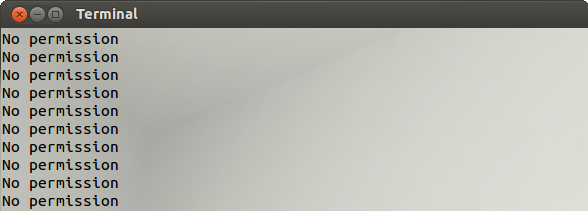
\includegraphics[width=0.9\linewidth]{noperm}
	\caption{Cannot Open File}
	\label{fig:noperm}
\end{figure}
\noindent In another terminal screen, we see the rapid switching of symlink endpoints. This shows that the attacking program is working as expected.
\begin{figure}[H]
	\centering
	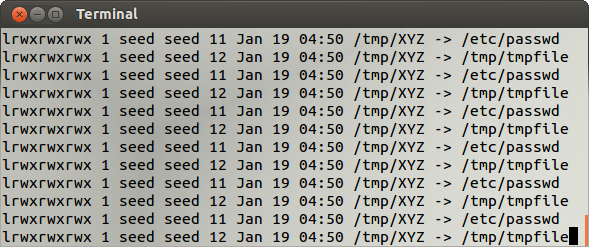
\includegraphics[width=0.9\linewidth]{rapidswitch}
	\caption{Rapid symlink Switching}
	\label{fig:rapidswitch}
\end{figure}
\noindent After some time, the bash script will stop running and show that the file has been modified. Upon inspection of the \texttt{/etc/passwd} file, the entry of an additional user account has been added. The last line in Figure 4 proves that the file has been modified to add our malicious user with user id 0 (root).
\begin{figure}[H]
	\centering
	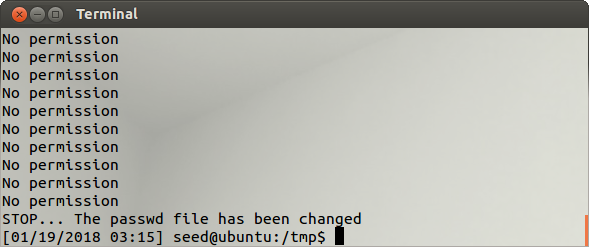
\includegraphics[width=0.9\linewidth]{editsuccess}
	\caption{Bash Stops After File Modified}
	\label{fig:editsuccess}
\end{figure}
\begin{figure}[H]
	\centering
	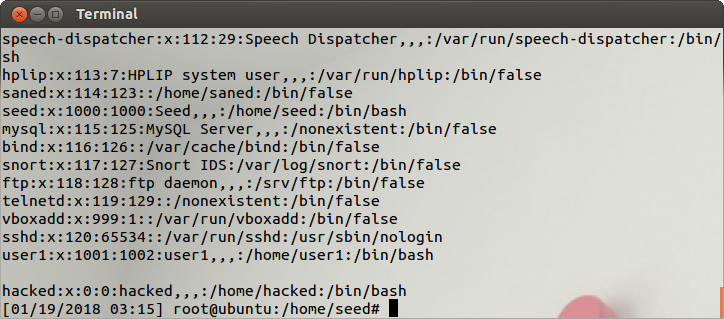
\includegraphics[width=0.9\linewidth]{passwdedit}
	\caption{Malicious User Added}
	\label{fig:passwdedit}
\end{figure}
\noindent We inspect our temporary file and find that the many repeated entries in the file were the failed attempts in trying to write into the privileged file during the symlink switching.
\begin{figure}[H]
	\centering
	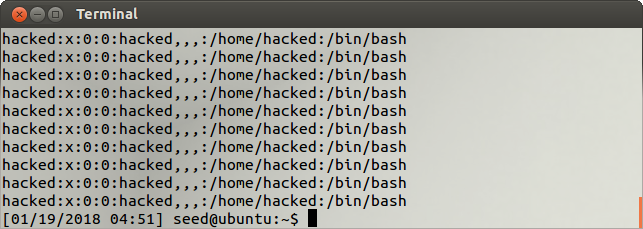
\includegraphics[width=0.9\linewidth]{tmpfile}
	\caption{Temporary File Contents}
	\label{fig:tmpfile}
\end{figure}
\noindent Before we are able to gain access to the account, the steps must be repeated for the \texttt{/etc/shadow} file. It is important to note that the \texttt{shadow} has a stricter privilege requirement and does not allow any non-root user to view the contents of the file, unlike the \texttt{passwd} file. Using the \texttt{cat} command as a standard user will throw the error ``Permission denied'' when reading \texttt{shadow}.\\\\The file containing the information to insert is edited and the program is run again. This time the success prompt is also shown after a few minutes. The file is examined with superuser and the specified data can be found inside the file.
\begin{figure}[H]
	\centering
	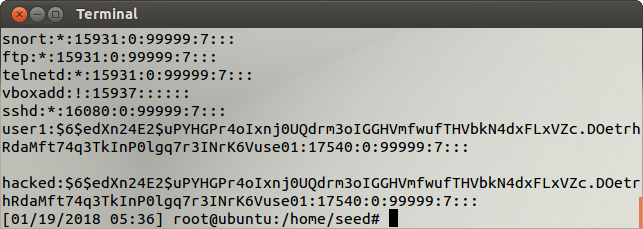
\includegraphics[width=0.9\linewidth]{shadowedit}
	\caption{File \texttt{shadow} Modified}
	\label{fig:shadowedit}
\end{figure}
\noindent To determine whether the procedure has been successful, we log in to our newly created user using the command \texttt{su <username>}. If successful, we will obtain root access. To check further, we navigate to the home directory of the user and print out the current directory using the command \texttt{pwd}.
\begin{verbatim}
$ su hacked
# cd ~
# pwd
\end{verbatim}
\begin{figure}[H]
	\centering
	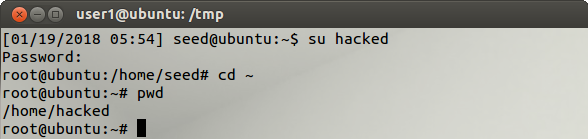
\includegraphics[width=0.9\linewidth]{hackedpwd}
	\caption{Root Access Obtained Using Existing Password}
	\label{fig:hackedpwd}
\end{figure}
From Figure 7, root access has been obtained and without the need of knowing the current system's superuser account. This exploit is fast to implement and the concept is simple. The next subsection will look into the difficulty of executing the same type of attack against introduction of additional guards for race conditions.
\subsection{Inode Checking}
To ensure it is harder for race conditions to be exploited, additional measures were implemented such as checking of inodes multiple times. These are cross-checked to ensure that the file being accessed is the same. The modifications to the vulnerable program have been attached in a separate subsection in the \hyperref[Appsec:3.3]{Appendix}.\\\\Even after the modifications and the programs are executed, we are still able to obtain a modified file. As we are not able to tell the order of execution of commands, it may be possible to obtain a modified privileged file although it may take a longer period of time to successfully pass all the checks.
\begin{figure}[H]
	\centering
	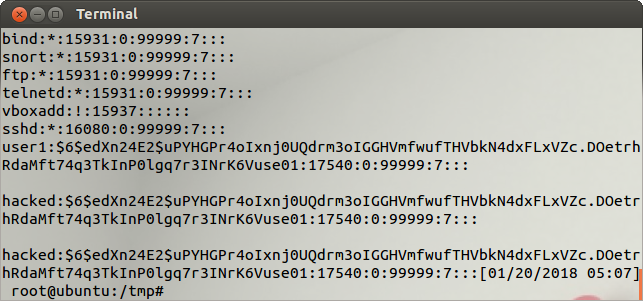
\includegraphics[width=0.9\linewidth]{hacked2x}
	\caption{Successful Despite Additional Protection}
	\label{fig:hacked2x}
\end{figure}
\subsection{Least Privilege}
The Principle of Least Privilege prevents the use of privileged access unless required and relinquished immediately after that. This prevents extended periods of access and loopholes being exploited when upgraded privileges are not required for the operation.\\\\In this task, we add a few lines to the code mainly to change the \texttt{euid} of the user. To restrict file access, \texttt{seteuid(getuid())} is used to forcibly downgrade the privileges of the user. The privileges are restored to root by using \texttt{seteuid(0)}. As the respective lines are added to the beginning and end of the program, the program will never be able to write into privileged files. This is due to the program not being able to access or open the file due to downgraded privileges. As such, this form of race condition exploit can be eliminated by carefully adjusting the access rights accordingly in the process of program execution.
\subsection{Sticky Symlinks Protection}
In this task, we look at the built-in protection scheme against following symlinks. Ubuntu versions 11.04 and above come with a built-in protection scheme against race condition attacks by activating sticky symlinks.\vspace{0.7em}
\begin{verbatim}
# sysctl -w kernel.yama.protected_sticky_symlinks=1
\end{verbatim}
\vspace{0.7em}
We perform the symlink this time pointing \texttt{"/tmp/XYZ"} to \texttt{"/home/seed/tmpfile"}. We note that the symlink is owned by the user, the euid is root and the directory is owned by root (since \texttt{"/tmp"} is world-writable). 
\begin{figure}[H]
	\centering
	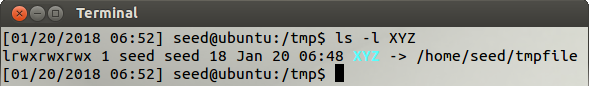
\includegraphics[width=0.9\linewidth]{symlinkperm}
	\caption{Symlink To Another User Controlled Directory}
	\label{fig:symlinkperm}
\end{figure}

\noindent If we were to execute the program, we will get ``Segmentation fault (core dumped)''. This is due to the sticky symlink protection. The symlink will not work if the following condition is satisfied.\\\\euid \texttt{==} Directory Owner \&\& euid\texttt{!=} Symlink Owner
\begin{figure}[H]
	\centering
	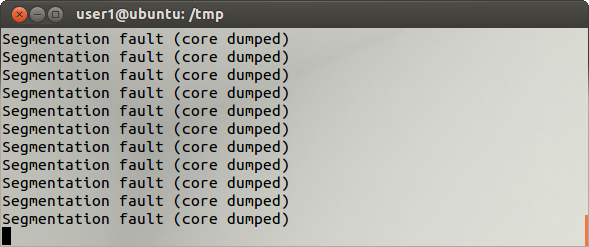
\includegraphics[width=0.9\linewidth]{symerror}
	\caption{Cannot Follow Symlink}
	\label{fig:symerror}
\end{figure}
\noindent \circled{1} This protection works because the euid is root and directory owner is also root, however the symlink owner is a different standard user. As a result, the symlink will never work when the sticky symlink option is turned on.
\\\\\circled{2} This is a good protection as it prevents world-writable folders such as \texttt{/tmp} to be used to mount a race condition exploit against privileged files. Furthermore, this also prevents files of other users from being modified as well.
\\\\\circled{3} The limitations of this scheme involve the actual root user being denied from being able to access user created symlinks although root users are supposed to be able to have full control of the system. Users opening up their own files through using their own symlinks will find that it is not possible if these users are using \texttt{Set-UID} programs. The following table shows the two conditions that users and root will be denied access if the symlink is created by a different user.
% Please add the following required packages to your document preamble:
% \usepackage[table,xcdraw]{xcolor}
% If you use beamer only pass "xcolor=table" option, i.e. \documentclass[xcolor=table]{beamer}
\begin{table}[H]
	\centering
	\label{symtab}
	\bgroup
	\def\arraystretch{1.3}
	\begin{tabular}{|c|c|c|c|}
		\hline
		euid & Directory Owner & Symlink Owner & fopen() \\ \hline
		seed & seed            & seed          & Allowed \\ \hline
		\rowcolor[HTML]{fffe65}
		seed & seed            & root          & Denied  \\ \hline
		seed & root            & seed          & Allowed \\ \hline
		seed & root            & root          & Allowed \\ \hline
		root & seed            & seed          & Allowed \\ \hline
		root & seed            & root          & Allowed \\ \hline
		\rowcolor[HTML]{fffe65} 
		root & root            & seed          & Denied  \\ \hline
		root & root            & root          & Allowed \\ \hline
	\end{tabular}
\egroup
\caption{Table of Symlinks Access Rights}
\end{table}

\newpage
 \section{Appendix}
 \subsection{Vulnerable Program: \texttt{vulp.c}}
 \label{Appsec:3.2}
 \begin{minted}{C}
#include <stdio.h>
#include <unistd.h>
#include <string.h>
 
int main()
{
    char* fn = "/tmp/XYZ";
    //char buffer[300]; //For /etc/shadow
    char buffer[60]; //For /etc/passwd
    FILE *fp;
    //originaleuid = geteuid(); //For task 3
    
    //seteuid(getuid); //For task 3
    /* Get user input */
    //scanf("%270s", buffer); //For /etc/shadow
    scanf("%50s", buffer); //For /etc/passwd
     
    if(!access(fn, W_OK)){
        fp = fopen(fn, "a+");
        fwrite("\n", sizeof(char), 1, fp);
        fwrite(buffer, sizeof(char), strlen(buffer), fp);
        fclose(fp);
    }
    else printf("No permission \n");
    //seteuid(originaleuid); //For task 3
}
 \end{minted}
  \subsection{Bash script}
  *The bash script, when created via Terminal usually has permission 664. The permission must be changed to 164, 364 or 764 for it to be executable.
 \begin{minted}{bash}
#!/bin/sh
 
old=`ls -l /etc/passwd`
new=`ls -l /etc/passwd`
 
while [ "$old" = "$new" ]
do
    new=`ls -l /etc/passwd`
    /tmp/vulp < /tmp/TXTFILE
done
echo "STOP... The passwd file has been changed"
 \end{minted}
 \newpage
  \subsection{Vulnerable Program with Inode Check: \texttt{vulp.c}}
  \label{Appsec:3.3}
 \begin{minted}{C}
#include <stdio.h>
#include <unistd.h>
#include <string.h>
#include <sys/types.h>
#include <sys/stat.h>
 
int main()
{
    noperm=1;
    char* fn = "/tmp/XYZ";
    //char buffer[300]; //For /etc/shadow
    char buffer[60]; //For /etc/passwd
    FILE *fp;
    struct stat before, mid, after;
 
    lstat("/tmp/XYZ", &before);
    /* Get user input */
    //scanf("%270s", buffer); //For /etc/shadow
    scanf("%50s", buffer); //For /etc/passwd
    lstat("/tmp/XYZ", &mid);
    if(!access(fn, W_OK))
        if(!access(fn, W_OK))
            if(!access(fn, W_OK)){
                lstat("/tmp/XYZ", &after);
                if(before.st_ino==after.st_ino && 
                before.st_ino==mid.st_ino){
                    fp = fopen(fn, "a+");
                    fwrite("\n", sizeof(char), 1, fp);
                    fwrite(buffer, sizeof(char), strlen(buffer), fp);
                    fclose(fp);
                    noperm=0;
                }
            }
    if(noperm) printf("No permission \n");
}
 \end{minted}

\end{document}